\documentclass[a4paper]{article}

\usepackage[portuguese]{babel}
\usepackage[utf8x]{inputenc}
\usepackage{amsmath}
\usepackage{graphicx}
\usepackage[colorinlistoftodos]{todonotes}

\title{Segundo Trabalho de Base de Dados}
\author{João Calhau - 31621 \\ Ricardo Benedito - 31643}

\begin{document}
\maketitle

\section{Introduction}
Com este projecto de Base de Dados vimos desenvolver um modelo E-R e a sua respectiva base de dados utilizando algebra relacional e PostgreSQL.

\newpage

\begin{figure}
\centering
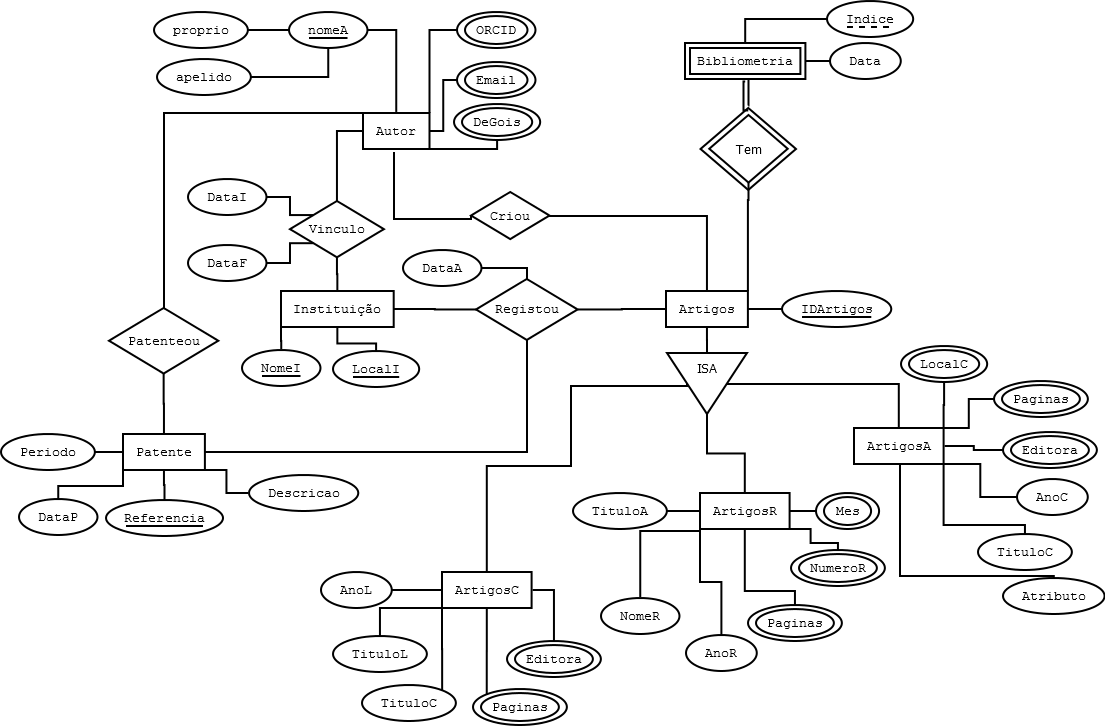
\includegraphics[width=1\textwidth]{Diagrama1.png}
\caption{Modelo E-R}
\label{overflow}
\end{figure}

\newpage

\section{Exercicios}
\subsection{Modelo E-R}
Podemos ver o desenho do modelo E-R na figura acima

\newpage
\subsection{Tabelas}
autor(\underline{Proprio}, \underline{Apelido})\\
autorORCID(\underline{Proprio}, \underline{Apelido}, ORCID)\\
autorEmail(\underline{Proprio}, \underline{Apelido}, Email)\\
autorDeGois(\underline{Proprio}, \underline{Apelido}, DeGois)\\
vinculo(\underline{Proprio}, \underline{Apelido}, \underline{NomeI}, \underline{LocalI}, dataI, dataF)\\
instituicao(\underline{NomeI}, \underline{LocalI})\\
criou(\underline{Proprio},\underline{Apelido}, \underline{IDArtigos})\\
registou(\underline{NomeI}, \underline{LocalI}, \underline{IDArtigos}, \underline{Referencia}, data)\\
patente(\underline{Referencia}, Periodo, Descricao, DadaP)\\
artigos(\underline{IDArtigos})\\
artigosC(\underline{IDArtigos}, TituloC, tituloL, AnoL)\\
artigosCP(\underline{IDArtigos}, paginas)\\
artigosCE(\underline{IDArtigos}, editora)\\
artigosR(\underline{IDArtigos}, TituloA, NomeR, AnoR)\\
artigosRP(\underline{IDArtigos}, Paginas)\\
artigosRM(\underline{IDArtigos}, Mes)\\
artigosRN(\underline{IDArtigos}, NumeroR)\\
artigosA(\underline{IDArtigos}, AnoC, TituloC, TituloR)\\
artigosAL(\underline{IDArtigos}, LocalC)\\
artigosAP(\underline{IDArtigos}, Paginas)\\
artigosAE(\underline{IDArtigos}, Editora)\\
patenteou(\underline{Proprio}, \underline{Apelido}, Referencia)\\
bibliometria(\underline{IDArtigos}, \underline{Indice}, DataB)\\
tem(\underline{IDArtigos}, \underline{IDArtigos}, \underline{Indice})\\

\newpage
\subsection{Dependencias Funcionais}

\newpage
\subsection{Cobertura Canónica}

\newpage
\subsection{Boyce-Codd}
Já está na forma normal de Boyce-Codd.

\subsection{Preservação de Dependencias}
Visto que já está na forma normal de Boyce-Codd, então não precisa de ser passado para a terceira forma normal.

\subsection{Chaves Primarias e afins}
As chaves primarias estão a sublinhado.\\
Tabela autor não tem chaves estrangeiras.\\
Tabela autorORCID tem Proprio e Apelido como chaves estrangeiras da tabela autor.\\
Tabela autorEmail tem Proprio e Apelido como chaves estrangeiras da tabela autor.\\
Tabela autorDeGois tem Proprio e Apelido como chaves estrangeiras da tabela autor.\\
Tabela vinculo tem Proprio e Apelido como chaves estrangeiras da tabela autor e NomeI e LocalI da tabela instituicao.\\
Tabela instituicao nao tem chaves estrangeiras.\\
Tabela criou tem Proprio e Apelido como chaves estrangeiras da tabela autor e IDArtigos da tabela artigos.\\
Tablea registou tem IDArtigos como chave estrangeira da tabela artigos, NomeI e LocalI da tabela instituicao e Referencia da tabela patente.\\
Tabela patente nao tem chaves estrangeiras.\\
Tabela Artigos nao tem chaves estrangeiras.\\
Todas as tabelas com o nome "artigos" tem IDArtigos como chave estrangeira da tabela artigos.\\
Tabela patenteou tem Proprio e Apelido como chaves estrangeiras da tabela autor e Referencia da tabela patente.\\
Tabela bibliometria tem chave estrangeira IDArtigos da tabela artigos.\\
Tabela tem tem IDartigos e indice como chaves estrangeiras da tabela bibliometria e IDArtigos da tabela artigos.\\

\newpage
\subsection{Criação das tabelas em SQL}
Comandos de criação das tabelas estão no ficheiro .txt que vem em conjunto com o pdf.

\subsection{Teste da Base de Dados}
Comandos de teste (Inserts) estão no ficheiro .txt que vem em conjunto com o pdf.

\subsection{Expressões em SQL}
As expressões em SQL estão também no ficheiro .txt que vem em conjunto com o pdf.
\end{document}